\section*{Введение}
% Такой заголовок пойдет в оглавление, только без нумерации
\addcontentsline{toc}{section}{Введение}


\clearpage
\section{Постановка задачи}

Принцип действия импульсного погружателя (рис. \ref{fig:scheme_porg}) основан на эффекте резкого снижения сопротивлению погружения свайного элемента при сообщении последнему вибрации. При вращении дисбалансов на их ось крепления действует центробежная сила и импульсный погружатель получает вибрирующее движение, которое сообщается свайному элементу через наголовник.

\begin{definition}
    Сила, препятствующая материальной точке, движущейся по окружности, удалиться от центра этой окружности, называется центростремительной силой. Она направлена по радиусу от окружности к центру. По третьему закону Ньютона имеется равная ей и противоположно направленная сила противодействия (сила, с которой движущаяся точка стремится удалиться от центра). Эта сила называется центробежной.
\end{definition}

\begin{definition}
    Импульсным погружением называют внедрение твердого тела в сопротивляющуюся среду под действием постоянной и знакопеременной сил.
\end{definition}

% \begin{definition}
%     Под вибрационным внедрением будем понимать внедрение твердого тела в сопротивляющуюся среду с заданной средней скоростью.
% \end{definition}

\begin{definition}
    Дебалансом называют неуравновешенность вращающихся частей машин (роторов, коленчатых валов, шкивов и т. п.).
\end{definition}

\begin{figure}[h]
    \centering
    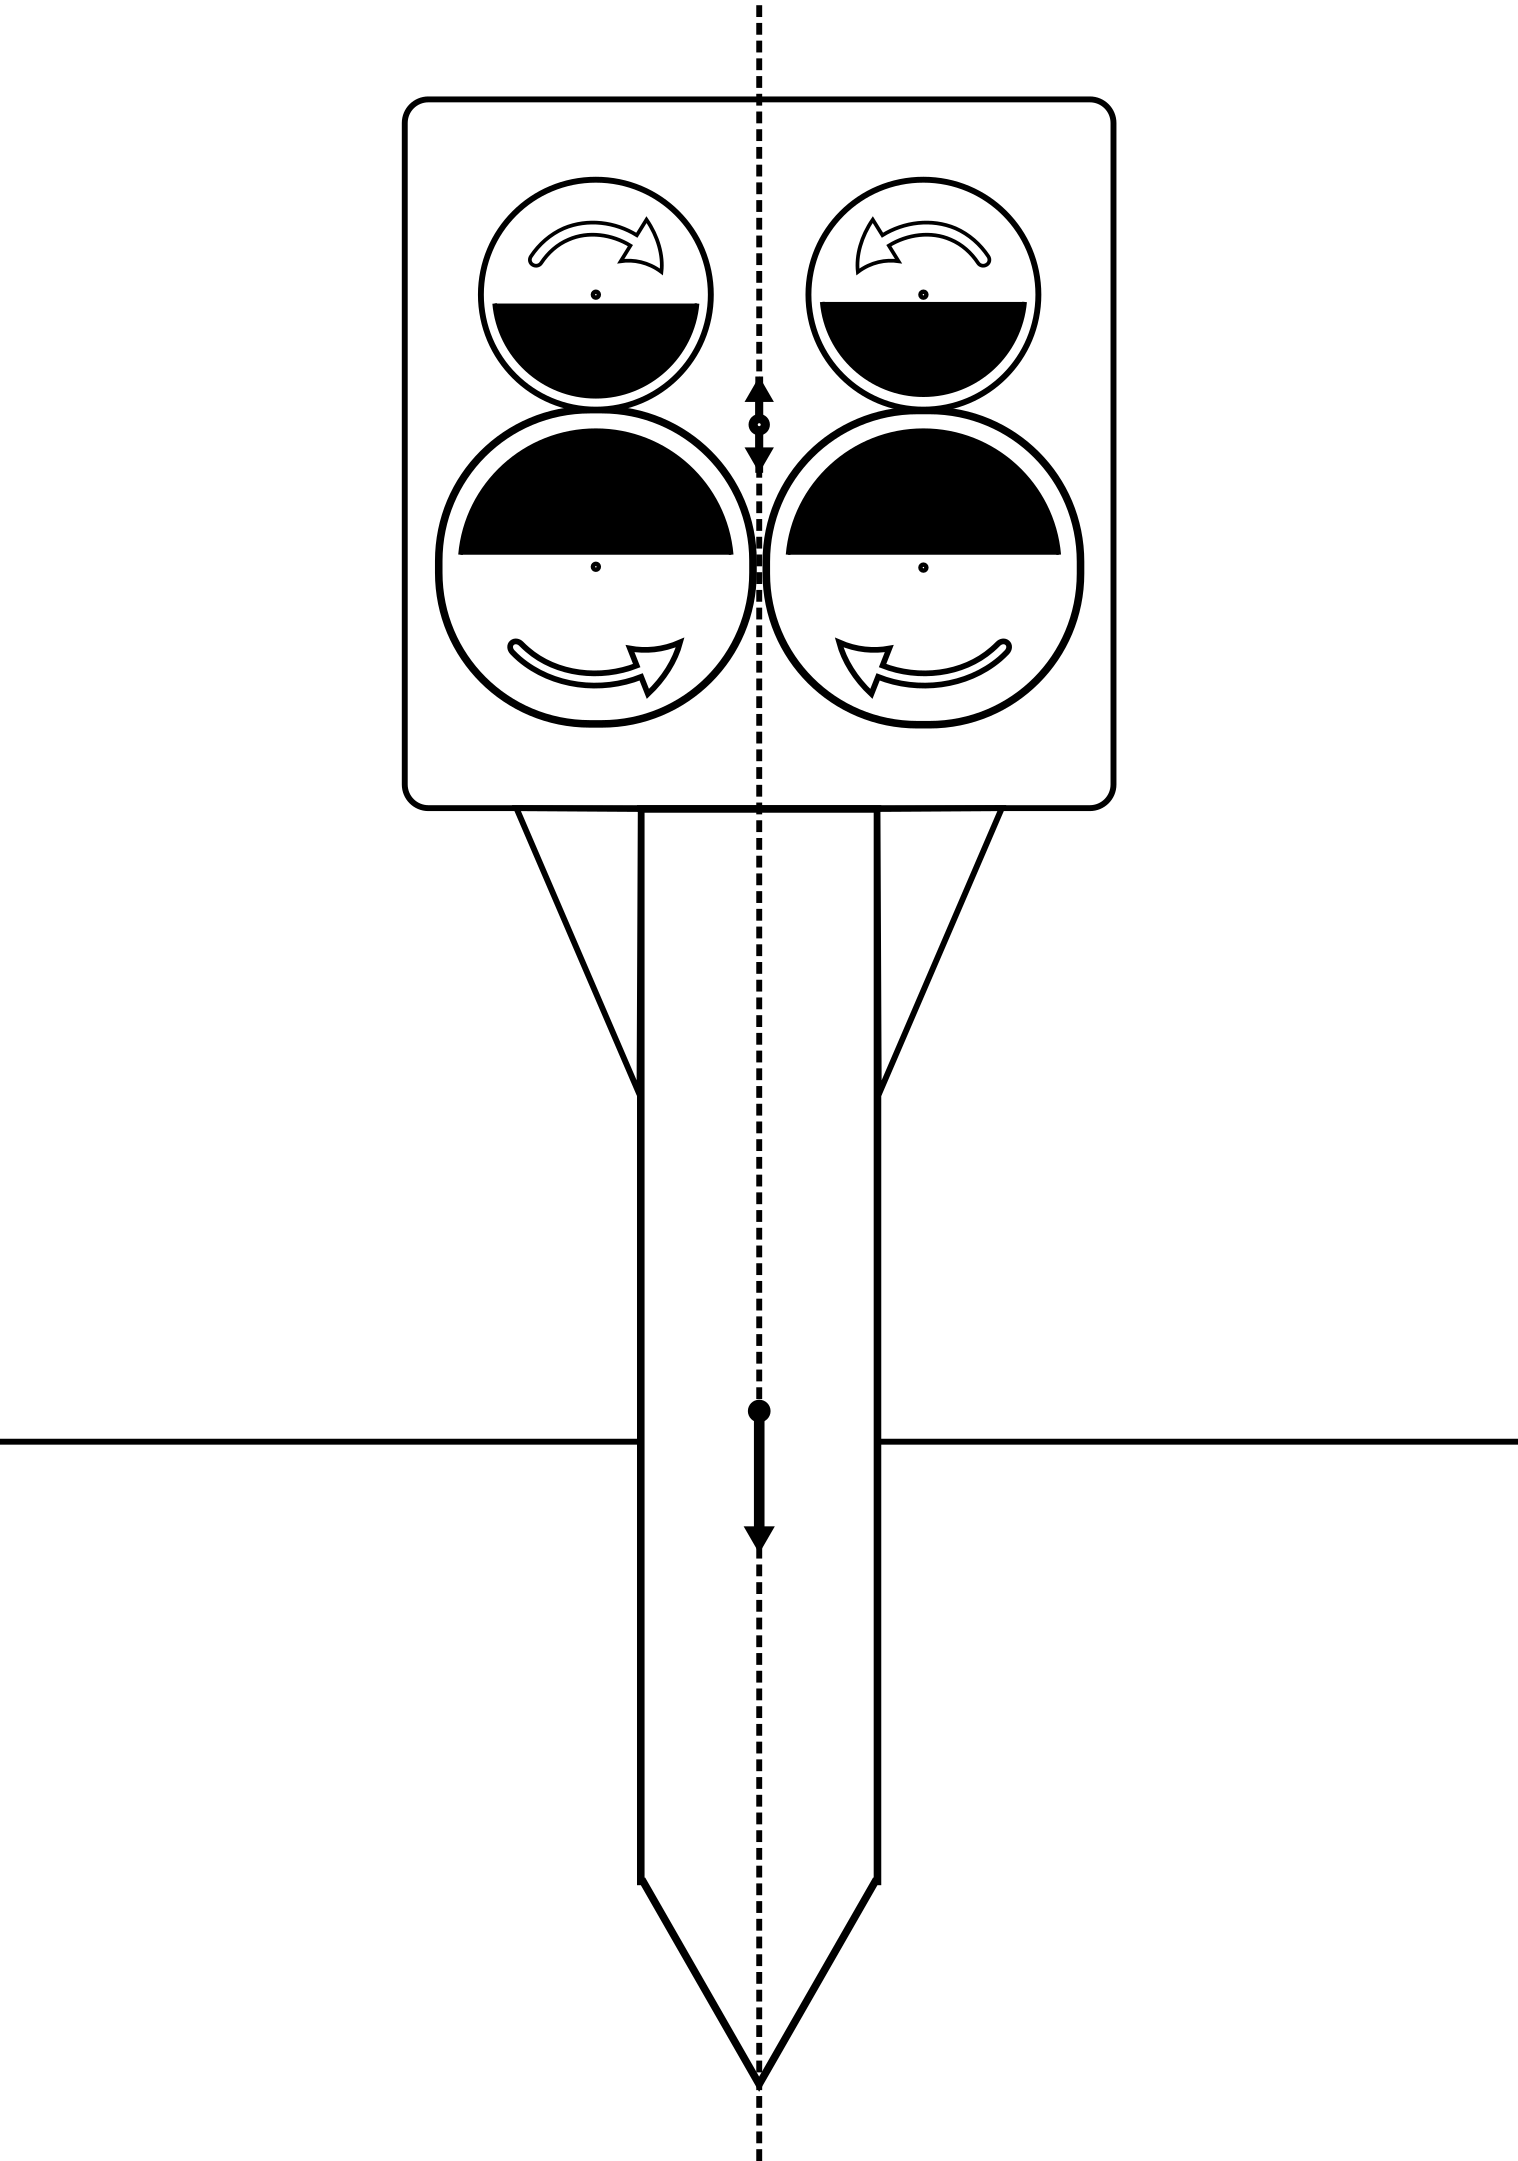
\includegraphics[width=0.5\linewidth]{img/scheme_porg.png}
    \caption{Схема импульсного погружателя.}
    \label{fig:scheme_porg}
\end{figure}


\clearpage
\section{Модель}

Пусть дан некий дебаланс с радиусом $r$, радиус вала которого равен $R$, $\omega$ --- угловая скорость и $l$ --- расстояние от центра масс до оси вращения дебаланса, а его масса будет равна $m$ (рис. \ref{fig:debalance}). 

\begin{figure}[h]
    \centering
    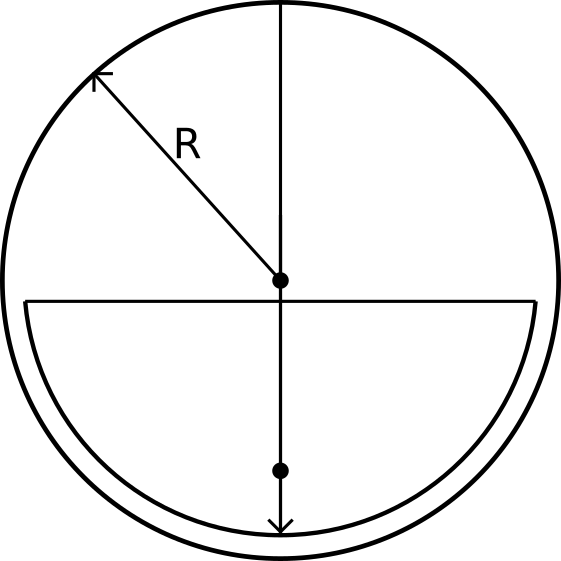
\includegraphics[width=0.4\linewidth]{img/debalance.png}
    \caption{Схема дебаланса.}
    \label{fig:debalance}
\end{figure}

Тогда, при вращении данного дебаланса возникнет центробежная сила, которая имеет вид:

\begin{equation}\label{eq:centrifugal}
    \begin{gathered}
        F_{\textrm{центр.}} = m \cdot \omega^2 \cdot l \\
        \textrm{где } l = ... , m = \rho \cdot V
    \end{gathered}
\end{equation}

Вращение такого дебаланса вокруг собственной оси будет иметь вид гармонического колебания.

\begin{definition}
    Гармоническим колебанием называют колебание, в процессе которого величины, характеризующие движение (смещение, скорость, ускорение и др.), изменяются по закону синуса или косинуса (гармоническому закону).
\end{definition}

Уравнение гармонического колебания дебаланса будет иметь вид:

\begin{equation}\label{eq:harmonic}
    \begin{gathered}
        x(t) = \lambda \cos (\omega t + \varphi_0) \\
        \textrm{где } \lambda = m \cdot \omega \cdot l
    \end{gathered}
\end{equation}

где $x(t)$  — значение изменяющейся величины в момент времени $t$, $\lambda$ — амплитуда колебаний, $\omega$ — циклическая (круговая) частота колебаний, $\varphi_0$ — начальная фаза колебаний.

Гармонические колебания являются периодическими. Период $T$ этих колебаний равен периоду функции $\cos (\omega t + \varphi_0)$, то есть:

\begin{equation*}
    \begin{aligned}
        T = \frac{2 \pi}{\omega}
    \end{aligned}
\end{equation*}

Начальная фаза колебаний в работе импульсного погружателя не является важной, из чего следует, что ее можно игнорировать [\ref{fn:kostin_work}]:

\footnotetext[1]{\label{fn:kostin_work} Пруфы на причину игнорирования начальная фаза колебаний...}

\begin{equation}\label{eq:harmonic_notphi}
    \begin{aligned}
        x(t) = \lambda \cos (\omega t)
    \end{aligned}
\end{equation}

В работе вибропогружателя полезной силой считается та, которая направлена на погружение твердого тела в сопротивляющуюся среду. Для компенсации сил, направленных перпендикулярно полезной силе, используются парные дебалансы, направление вращения которых в разные стороны, по отношении друг к другу (рис. \ref{fig:scheme_porg}). В таком случае, уравнение гармонического колебания будет иметь вид:

\begin{equation}\label{eq:harmonic_dual}
    \begin{aligned}
        x(t) = 2 m \omega^2 l \cos (\omega t)
    \end{aligned}
\end{equation}

Сила, направленная вверх может привести к разрушению твердого тела. Для компенсации этой силы в импульсного погружателе используется несколько пар дебалансов разного радиуса.

Уравнение гармонического колебания для второй пары дебалансов будет иметь вид:

\begin{equation*}
    \begin{aligned}
        x(t) = 2 m_2 \cdot 4 \omega^2 \cdot l(r_2) \cdot \cos (2 \omega t)
    \end{aligned}
\end{equation*}

Уравнение гармонического колебания для пары дебалансов в общем виде:

\begin{equation}\label{eq:harmonic_common}
    \begin{aligned}
        x(t) = 2 m_k \cdot (k \omega)^2 \cdot l(r_k) \cdot \cos (k \omega t)
    \end{aligned}
\end{equation}

Для всех пар дебалансов сумма гармонических колебаний будет иметь вид:

\begin{equation}\label{eq:harmonic_sum}
    \begin{gathered}
        F = \sum_{k = 1}^{n} 2 m_k \cdot (k \omega)^2 \cdot l(r_k) \cdot \cos (k \omega t) \\
        \textrm{где $n$ --- количество пар дебалансов} 
    \end{gathered}
\end{equation}

Импульс силы для двух пар дебалансов за время $t$ представлен на графике (\ref{grap:impulse}).

\begin{definition}
    Импульсом силы называют векторную физическую величину, которая является мерой действия силы за некоторый промежуток времени. $\vec{I}$ --- импульс силы $\vec{F}$ за малый промежуток времени $t$.
\end{definition}

\begin{figure}[h]
    \centering
    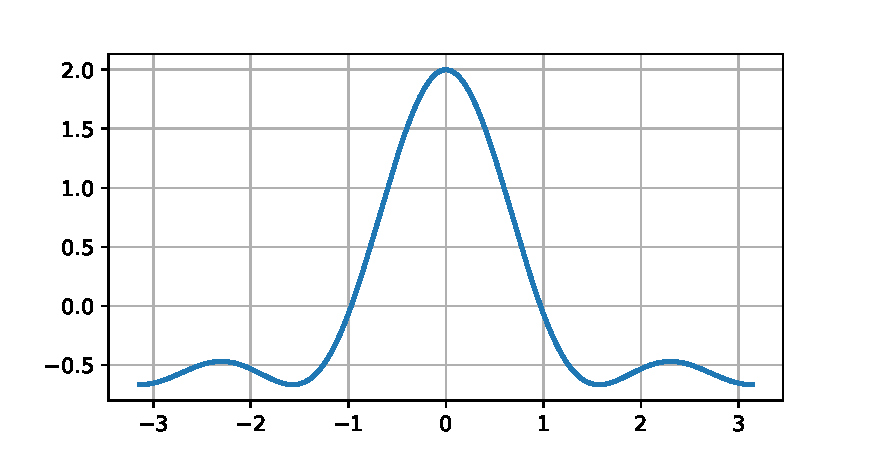
\includegraphics[width=1\linewidth]{grap/impulse.pdf}
    \caption{Импульс силы для трех пар дебалансов.}
    \label{grap:impulse}
\end{figure}


\clearpage
\section{Задача оптимизации}

Для получения наибольшего импульса силы для погружения твердого тела в сопротивляющуюся среду и компенсации силы, которая направлена в противоположную сторону, необходимо подобрать оптимальное соотношение характеристик пар дебалансов между собой.

Сформулируем задачу оптимальности. Пусть $f_{\max}(t)$ --- максимальное значение импульса силы за время $t$, $f_{\min}(t)$ --- минимальное значение импульса за время $t$. Тогда:

\begin{equation}\label{eq:optim}
    \begin{aligned}
        K = \left| \frac{f_{\max}(t)}{f_{\min}(t)} \right| \rightarrow \max
    \end{aligned}
\end{equation}

Исходя из теоремы оптимальности модели полигармонического импульса [\ref{fn:kostin_work}] многочлен (\ref{eq:harmonic_sum}) является оптимальным тогда и только тогда, когда он с точностью до постоянного множителя имеет вид суммы Фейера

\footnotetext[2]{\label{fn:kostin_work} Д. В. Костин: Бифуркации резонансных колебаний и оптимизация тригонометрического импульса по коэффициенту несимметрии}

\begin{equation}\label{eq:feer}
    \begin{gathered}
        f_n(t) = \sum \limits_{k=1}^n (n+1-k) \cos(kt) \\
        \textrm{При этом имеет место равенство:} \\
        \max \limits_{\lambda} K_n(\lambda) = n
    \end{gathered}
\end{equation}

Из этого следует, что:

\begin{equation}\label{eq:opt_attitude}
    \begin{gathered}
        \lambda_k = \frac{n - k + 1}{n} \\
        \textrm{где $n$ - количество пар дебалансов,} \\
        \textrm{$k$ - порядковый номер пары дебалансов}
    \end{gathered}
\end{equation}

Выражение (\ref{eq:opt_attitude}) дает возможность оптимизации характеристик каждой пары дебалансов в импульсном погружателе для получения наибольшего импульса силы для погружения твердого тела и компенсации силы, которая направлена в противоположную сторону.


\clearpage
\section{Заключение}


\clearpage
\section{Приложение}
\subsection{Исходный код main.py}
% \lstinputlisting[language=Python, breaklines]{code/app.py}


\clearpage
\addcontentsline{toc}{section}{Список литературы}
\begin{thebibliography}{}
    \bibitem{}
\end{thebibliography}
